\documentclass[11pt]{article}
\usepackage[margin=1in]{geometry}
\usepackage[numbers,sort&compress]{natbib}
\usepackage{graphicx}
\usepackage{booktabs}
\usepackage{amsmath,amssymb}
\usepackage{microtype}
\usepackage[colorlinks=true,linkcolor=blue,citecolor=blue,urlcolor=blue]{hyperref}

\newcommand{\de}{\Delta E_{00}}
\newcommand{\Wp}{W^{+}}

\title{A Zero-Parameter Latent Color Operator:\\
Photometric Equivariance for Diffusion Tokenizers}
\author{Rashed Almansouri\\
\small Brown University\\
\small \texttt{rashed\_almansouri@brown.edu}}
\date{}

\begin{document}
\maketitle

\begin{abstract}
We derive a \emph{zero-parameter, closed-form} latent-space operator for
photometric transforms brightness, contrast, saturation, hue on diffusion
tokenizers. These transforms, unlike the spatial warps of prior equivariance
work, have no canonical action on the latent grid. We canonicalize this
augmentation family as a subgroup of the pointwise color-affine group
$\mathrm{Aff}(3)$ and obtain the operator by conjugating the pixel-space
action through the fitted linear latent-to-RGB map of SD-VAE. On the frozen autoencoder this
operator steers brightness, contrast, and saturation roughly $2\times$ past the
do-nothing floor but fails entirely on hue, even though a per-image
decoder-inversion oracle shows every factor is decoder-expressible
($\de$ ceilings $1.7$--$5.5$). Twenty thousand steps of decoder-routed
equivariance fine-tuning close this gap: the closed-form operator reaches
$\de$ $4.4$--$4.9$ on \emph{all four} factors closing $0.76$--$0.92$ of
the oracle gap against a compute-matched control at a cost of
$0.31$\,dB PSNR. Learned operators
(a Lie-algebra parameterization and a strictly more expressive convolutional
variant) provide no consistent overall advantage, and an intervention that matches the
latent spectrum without the equivariance constraint confers none of the
equivariance. Diffusion transformers trained on the equivariant latents
converge faster at two model scales ($27\%$ lower FID at the 40K checkpoint
for DiT-S; $14$--$18\%$ at 30--40K for DiT-B, replicated across two seeds)
with equal final quality.
\end{abstract}

\section{Introduction}

Latent diffusion models~\citep{rombach2022ldm,peebles2023dit} generate in the
latent space of a pretrained autoencoder, and a growing body of work shows that
the \emph{structure} of that latent space not only its reconstruction
quality governs how fast and how well diffusion trains. EQ-VAE
\citep{kouzelis2025eqvae} demonstrated that fine-tuning the autoencoder so that
\emph{spatial} transforms of the image (scaling, $90^\circ$ rotation)
correspond to the same transforms applied directly to the latent grid yields
large diffusion speedups. Parallel work regularizes for scale
\citep{skorokhodov2025diffusability} and shift \citep{zhou2025afldm}
equivariance. In every one of these cases the latent operator is
\emph{inherited}: a spatial warp of an image has an obvious counterpart on the
spatially downsampled latent.

Photometric transforms break this pattern. A brightness change, a saturation
shift, or a hue rotation acts pointwise on RGB values, and a diffusion
tokenizer's latent channels are not RGB: there is no canonical answer to the
question \emph{``what does a hue shift do to a latent?''} This paper treats
that missing operator as the central object of study.

\paragraph{Contributions.}
\begin{enumerate}
  \item \textbf{A closed-form latent color operator.} We canonicalize the
  standard photometric family (brightness, fixed-anchor contrast, saturation,
  hue) as a subgroup/monoid of $\mathrm{Aff}(3)$, prove an exact
  photometric--spatial commutation lemma, and derive a zero-parameter latent
  operator $M_a = \Wp A_a W + (I - \Wp W)K$ from the fitted linear
  latent-to-RGB map $W$, with an explicit treatment of $W$'s null space
  (Section~\ref{sec:method}).
  \item \textbf{An oracle methodology.} Per-image decoder inversion gives, for
  each transform, the best equivariance error \emph{any} latent edit could
  achieve. This turns the headline result into a fraction of the achievable
  rather than a raw error, and separates two failure modes that are otherwise
  confounded: on the frozen SD-VAE, hue is decoder-expressible
  ($\de \approx 2.9$ oracle) yet unreachable by affine steering
  (at the do-nothing floor).
  \item \textbf{The closed form is sufficient once the autoencoder
  cooperates.} Brief decoder-routed fine-tuning makes the closed-form operator
  approach the oracle ceiling on all four factors, including hue. A learned
  Lie-algebra operator, its ablations, and a convolutional operator with
  $90$K parameters provide no consistent overall advantage over it. Single-factor training
  reveals a structured transfer pattern; and a spectral-matched intervention
  shows that, at the representation level, the equivariance is not a side
  effect of latent spectral statistics.
  \item \textbf{Faster diffusion convergence at two scales.} DiT-S and DiT-B
  trained on the equivariant latents reach mid-training FID milestones
  substantially earlier than compute-matched controls, echoing at the
  photometric level the convergence benefits previously reported for spatial
  equivariance, with endpoint quality unchanged (two seeds per arm at the
  larger scale).
\end{enumerate}

\section{Related Work}
\label{sec:related}

\paragraph{Equivariance regularization of diffusion latents.}
EQ-VAE \citep{kouzelis2025eqvae} fine-tunes pretrained autoencoders so that
scaling and $90^\circ$ rotations of the input correspond to grid operations on
the latent, routing the constraint through the decoder after observing that
explicit latent matching collapses the representation; we inherit both the
loss structure and that constraint. \citet{skorokhodov2025diffusability}
regularize for scale equivariance via joint downsampling;
\citet{zhou2025afldm} for shift equivariance. DC-AE~1.5
\citep{chen2025dcae15} structures latents by channel-wise masking and
explicitly forgoes equivariance; VA-VAE \citep{yao2025vavae} aligns latents
with vision foundation models. All prior equivariance work in this line is
spatial; the operator-design problem that photometric transforms pose is, to
our knowledge, unaddressed.

\paragraph{Learned group actions and color equivariance.}
The Homomorphism AutoEncoder \citep{keurti2023hae} learns a group
representation acting on the latent of a small autoencoder trained from
scratch on group-structured data; our learned baseline transplants this idea
onto a production-scale tokenizer (and finds it unnecessary). CEConv
\citep{lengyel2023ceconv} builds hue equivariance into network architecture
for discriminative tasks; we instead regularize a pretrained tokenizer,
requiring no architectural change.

\paragraph{Skepticism about equivariance as a latent property.}
\citet{zhong2026rightspace} report, across 86 heterogeneous tokenizers, that
an affine-equivariance metric correlates weakly with diffusion quality. Our
setting complements theirs: we hold architecture, data, and compute fixed,
vary only the constraint, and include a spectral-matched intervention, an
in-family interventional probe rather than a cross-family correlation.

\section{Method}
\label{sec:method}

\subsection{A canonicalized photometric family}
\label{sec:family}

We work with pixel colors $x_p \in \mathbb{R}^3$ and define the photometric
family as pointwise color-affine maps $\tau_a(x)_p = A_a x_p + b_a$ with
$a = (A_a, b_a) \in \mathrm{Aff}(3)$. The standard augmentation factors embed
as one-parameter families: \emph{brightness} $A=\beta I$; \emph{contrast}
$A=\gamma I$, $b=(1-\gamma)g\mathbf{1}$ anchored at fixed gray $g=0.5$;
\emph{saturation} $A = sI + (1-s)\mathbf{1}w^\top$ with BT.601 luma weights
$w$; \emph{hue} a rotation $R(\theta)$ about the luma axis (YIQ convention).
Two canonicalizations are load-bearing. First, library implementations of
contrast use the \emph{image-dependent} mean gray, which is not a pointwise
map and breaks composition; the fixed anchor restores an exact group law.
Second, saturation is a \emph{monoid} with a non-invertible absorbing element
at $s{=}0$ (grayscale). Equivariance targets are computed before clipping to
$[0,1]$; we measure the clipped-pixel fraction rather than assuming it small
(it reaches $20$--$27\%$ at the extremes of the widest ranges, which is why
training uses $\beta,\gamma \in [0.7, 1.3]$).

For any pointwise-affine latent map $T$ and any spatial warp $S$ implemented
with convex-combination interpolation, $T \circ S = S \circ T$ exactly, since
affine maps commute with convex combinations. Photometric latent operators
therefore compose freely with the spatial operators of prior work, without
ordering ambiguity.

\subsection{The closed-form operator}
\label{sec:closedform}

SD-VAE latents $z \in \mathbb{R}^{4 \times 32 \times 32}$ admit a well-known
approximate linear color decoding $\hat{x}_p \approx W z_p + c$; we re-fit
$(W, c)$ by least squares on $1{,}024$ OpenImages validation images and obtain
$R^2 = 0.859$ (per channel $0.844/0.890/0.847$). If decoding were exactly this
pointwise map, equivariance $D(T_a z) = \tau_a(D(z))$ would force, per latent
site, $W T_a(z_p) + c = A_a(Wz_p + c) + b_a$. Solving for a channel-affine
$T_a(z_p) = M_a z_p + m_a$ with $W$ of full row rank yields
\begin{equation}
\label{eq:closedform}
M_a \;=\; \Wp A_a W \;+\; (I - \Wp W)\,K,
\qquad
m_a \;=\; \Wp\!\left(A_a c + b_a - c\right),
\end{equation}
where $\Wp$ is the Moore--Penrose pseudo-inverse and $K$ acts on the one-dimensional subspace invisible to the fitted linear RGB probe. We use $K = I$ (identity on the residual subspace), for which the
homomorphism $M_{a \circ b} = M_a M_b$ holds exactly on the color block. The
operator has \emph{no trainable parameters}: for a sampled transform, compose
the factor matrices in homogeneous coordinates and apply
Eq.~\eqref{eq:closedform}.

\subsection{Decoder-routed equivariance training}
\label{sec:training}

Following \citet{kouzelis2025eqvae}, the constraint reaches the latent only
through the decoder: with probability $p{=}0.5$ per sample we replace the
reconstruction objective by
$\mathcal{L}_\text{rec}\!\left(\tau_a(x),\, D(T_a(E(x)))\right)$, never
including any latent-matching term (the documented collapse mode). The
posterior is pushed forward through the affine operator analytically (mean
$M_a \mu + m_a$; marginal standard deviation
$\sqrt{\mathrm{diag}(M_a\,\mathrm{diag}(\sigma^2)\,M_a^\top)}$), and the KL
term is computed on the untransformed posterior. The fine-tune is GAN-free
($\ell_1$ + LPIPS + KL), 20K steps at batch 8, AdamW $10^{-4}$.

\subsection{The oracle: decoder-inversion ceilings}
\label{sec:oracle}

For each factor and magnitude we optimize a latent $z'$ directly to render the
transformed target, $\min_{z'} \lVert D(z') - \tau_a(x) \rVert^2$ (500 Adam
steps, 16 images). The resulting error is the decoder's expressivity
ceiling which is an empirical upper bound from unconstrained per-image latent optimization and the $R^2$ of a
channel-affine fit from $E(x)$ to $z'$ measures how affine the oracle's edit
is. Oracle edits are not unique, so this $R^2$ is a lower bound on affine
representability.

\section{Experiments}
\label{sec:experiments}

\subsection{Setup}
All experiments use SD-VAE (\texttt{sd-vae-ft-mse}, $f{=}8$, 4 channels) and
the OpenImages validation split ($41{,}620$ images at $256^2$;
\citealp{kuznetsova2020openimages}). Equivariance error (EE) is the
decoder-side discrepancy $\de\!\left(D(T_a E(x)),\, \tau_a(x)\right)$ in
CIEDE2000 \citep{sharma2005ciede2000}, averaged over a factor-specific grid
including held-out magnitudes and held-out compositions; CIEDE2000 is used for
color-fidelity thresholds because LPIPS is comparatively insensitive to smooth
global color shifts. Reconstruction is reported as PSNR and rFID at
$n{=}1{,}024$ (comparable across rows only). Every fine-tuned condition,
including the control \textsc{b1}, receives identical steps and losses; the
frozen autoencoder \textsc{b0} is a reference row, never the comparison
baseline. Seed repeats of \textsc{b1} and \textsc{p1} agree within
$0.3$--$0.6$ $\de$ per factor.

\subsection{Tier 0: the frozen autoencoder}
\label{sec:tier0}

On the frozen SD-VAE the closed-form operator beats the do-nothing floor by
roughly $2\times$ for brightness ($7.9$ vs.\ $17.0$ $\de$ at $\beta{=}0.6$),
contrast ($5.4$ vs.\ $9.2$), and saturation ($7.3$ vs.\ $12.6$ at $s{=}0$),
but sits \emph{at} the floor for hue ($13.0$ vs.\ $14.4$ at $-45^\circ$). The
oracle explains why this is an operator problem rather than a decoder problem:
inversion reaches $\de$ $2.2$--$5.5$ across factors and magnitudes (hue:
$2.8$--$2.9$ at $\pm 45^\circ$) so every factor is decoder-expressible and the
oracle's latent edits are $79$--$90\%$ channel-affine, with magnitude rather
than factor driving the non-affinity.

\subsection{Fine-tuning closes the gap with a zero-parameter operator}
\label{sec:main}

\begin{table}[t]
\centering
\small
\caption{Equivariance error (mean $\de$, lower is better) and reconstruction
after 20K fine-tuning steps. All rows except \textsc{b0} are compute-matched.
Stored-$W$ operator evaluation; the fair \textsc{b1} reference for gap-closed
uses a re-fitted $W$ reference $15.5/9.6/14.5/16.3$ (see text), not the
stored-$W$ \textsc{b1} row. Bold: best per column. Seed repeats put the
per-factor spread at $\pm 0.3$--$0.6$\,$\de$, so smaller differences are not
meaningful; among the photometric conditions, brightness is the only factor
on which the closed form separates from the learned variants beyond that
noise.}
\label{tab:main}
\begin{tabular}{lccccccc}
\toprule
Condition & Bright. & Contr. & Sat. & Hue & Composed & PSNR & rFID \\
\midrule
\textsc{b0} (frozen)            & 7.24 & 5.71 & 7.04 & 10.21 & 5.15 & 25.35 & 13.7 \\
\textsc{b1} (control)           & 31.6 & 11.6 & 23.6 & 24.6 & 17.4 & 25.34 & 17.3 \\
\textsc{b2lite} (spatial)       & 29.5 & 10.6 & 21.7 & 23.0 & 15.6 & 24.71 & 19.0 \\
\textsc{c1proxy} (spectral)     & 35.9 & 16.5 & 28.9 & 33.7 & 22.2 & 25.12 & 18.0 \\
\midrule
\textsc{p1} (closed form)       & \textbf{4.59} & 4.58 & 4.40 & 4.92 & 4.10 & 25.03 & 18.4 \\
\textsc{p2} (learned Lie)       & 6.50 & 5.01 & 5.70 & 4.95 & 4.47 & 25.08 & 18.0 \\
\textsc{p2}$-$comp.\ loss       & 6.44 & 4.81 & 5.08 & \textbf{4.52} & 4.04 & 25.11 & 17.6 \\
\textsc{p2}$-$analytic init     & 6.26 & \textbf{4.49} & 4.34 & 4.82 & \textbf{3.93} & 25.20 & 18.1 \\
\textsc{p3} (conv, 90K params)  & 10.0 & 4.75 & \textbf{3.81} & 4.65 & \textbf{3.93} & 25.22 & 17.8 \\
\midrule
Oracle ceiling (frozen)         & 2.2--5.5 & 2.1--4.3 & 1.7--3.0 & 2.8--2.9 & --- & --- & --- \\
\bottomrule
\end{tabular}
\end{table}

Table~\ref{tab:main} is the main result. After fine-tuning, the closed-form
operator reaches $\de$ $4.4$--$4.9$ on all four factors hue drops from
worse-than-nothing to $4.92$, closing $82\%$ of the gap to its $2.9$
frozen-decoder oracle ceiling at a reconstruction cost of $0.31$\,dB PSNR
against the control.
Because plain fine-tuning itself drifts the latent color geometry (the
control's EE under a $W$ re-fitted on its own latents is $15.5/9.6/14.5/16.3$),
we compute the headline \emph{gap-closed} fraction
$(\text{EE}_{\textsc{b1}} - \text{EE}_{\textsc{p1}}) /
(\text{EE}_{\textsc{b1}} - \text{EE}_\text{oracle})$ against that re-fitted
reference, with all three terms averaged over the magnitudes at which the
oracle was run (the range endpoints, where \textsc{p1}'s EE is
$4.8/4.7/4.6/5.3$): $0.92 / 0.76 / 0.82 / 0.82$ per factor.

Three additional observations. (i)~The spatial condition \textsc{b2lite}
validates the training loop against the known effect direction (its
\emph{spatial} EE is $6.1$ vs.\ the control's $10.5$) while leaving
photometric EE essentially unchanged as spatial equivariance does not
incidentally confer photometric equivariance. (ii)~All fine-tunes cost rFID relative to the
frozen \textsc{b0} ($13.7 \to 17$--$19$): the GAN-free recipe's price, shared
equally by the control. (iii)~Photometric training mildly degrades spatial EE
($13.5$ vs.\ $10.5$), so the two equivariances trade off rather than come for
free together.

\paragraph{What does not help.}
None of the added mechanisms we tested provide consistent overall advantage over the closed form. The
learned Lie operator matches the closed form on hue and is slightly worse
elsewhere; removing its composition loss or analytic initialization changes
nothing beyond seed noise; and the $90$K-parameter convolutional operator
improves saturation slightly while degrading brightness ($10.0$ vs.\ $4.6$) so no evidence the
latent color action is spatially heterogeneous.

\paragraph{Single-factor transfer.}
Training on one factor reaches near-ceiling on that factor (dedicated hue:
$4.40$, the best hue of any run) and transfers partially to the others
($2$--$4\times$ better than the control everywhere) without reaching their
ceilings; brightness training transfers near-ceiling to contrast (both are
diagonal scalings), while nothing transfers fully to hue (the chroma
rotation). The transfer pattern respects the algebra of
Section~\ref{sec:family}. Notably, single-factor runs pay no measurable
reconstruction cost.

\subsection{Mechanism: an intervention, not a correlation}
\label{sec:mechanism}

A natural deflationary hypothesis, prompted by \citet{zhong2026rightspace}, is
that equivariance training merely smooths latent statistics.
\textsc{c1proxy} tests this by intervention: it fine-tunes with a spectral
regularizer matched to \textsc{p1}'s measured latent spectrum
(achieved: slope $-0.821$ vs.\ $-0.832$; high-frequency fraction $0.0248$
vs.\ $0.0247$) and \emph{no} equivariance constraint. Its photometric EE is
worse than the control's on every factor under the fair re-fitted-$W$
protocol ($18.2/10.5/22.9/20.6$ vs.\ $15.5/9.6/14.5/16.3$;
Table~\ref{tab:main}). Matching the
spectrum confers none of the equivariance at the representation level, the
effect is not spectrally mediated. A complementary diagnostic tells the same
story: the linear latent-to-RGB fit quality $R^2$ falls from $0.86$ (frozen)
to $0.65$ under plain fine-tuning, is \emph{preserved} at $0.79$ by
equivariance training, and is destroyed hardest ($0.55$) by the
spectral-only regularizer.

\subsection{Generation: convergence at two scales}
\label{sec:generation}

\begin{figure}[t]
\centering
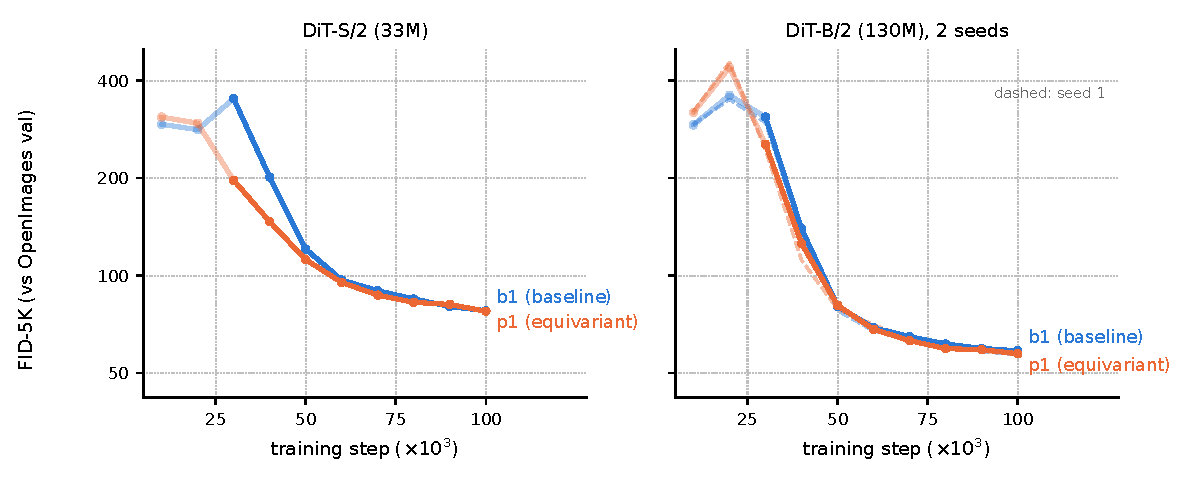
\includegraphics[width=\linewidth]{figures/fig_convergence.pdf}
\caption{FID-5K versus training step for diffusion transformers trained on
control (\textsc{b1}) versus photometric-equivariant (\textsc{p1}) latents,
at two model scales. Unconditional generation on OpenImages latents,
cfg-free DDPM sampling; points below 30K steps are shown at reduced opacity
(early FID-5K is noisy in both arms). DiT-B shows two seeds per arm (dashed:
seed 1); DiT-S one seed.}
\label{fig:convergence}
\end{figure}

\begin{figure}[t]
\centering
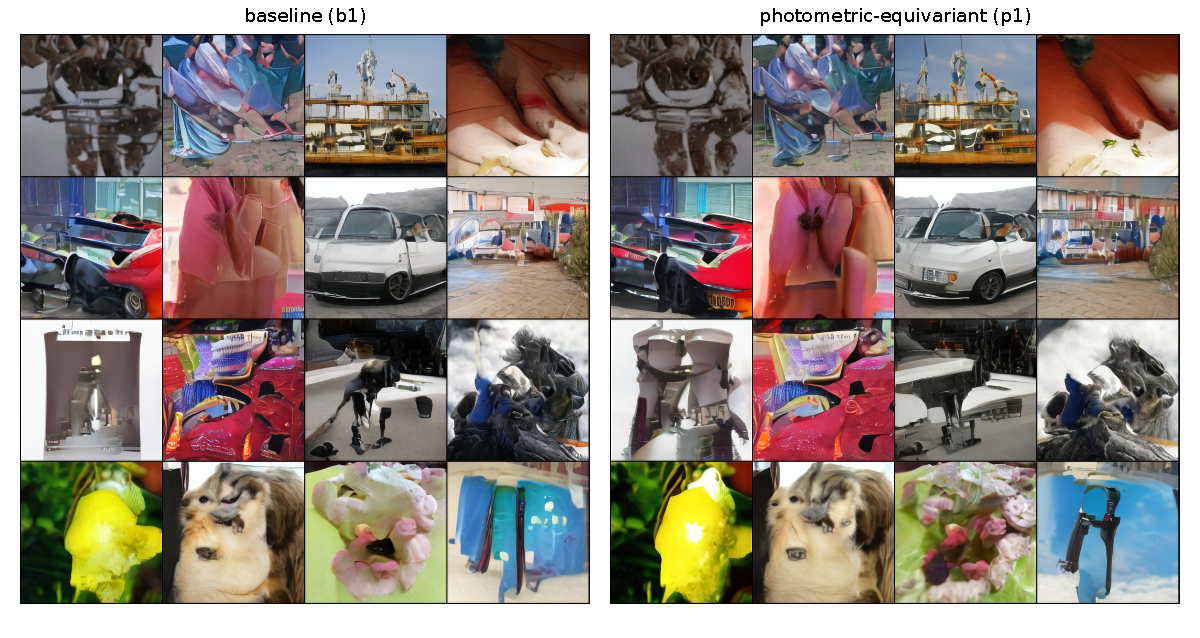
\includegraphics[width=\linewidth]{figures/fig_grids.pdf}
\caption{Seed-paired samples at 100K steps (DiT-B). Left: control latents;
right: photometric-equivariant latents.}
\label{fig:grids}
\end{figure}

We train unconditional DiT-S/2 (33M) and DiT-B/2 (130M)
\citep{peebles2023dit} for 100K steps on cached latents of \textsc{b1} and
\textsc{p1}, identical hyperparameters, FID-5K \citep{parmar2022cleanfid}
every 10K steps against a fixed reference of $10$K identically processed
OpenImages images (Figure~\ref{fig:convergence}). The reference is drawn
from the same $41$K-image pool the DiTs train on---no disjoint split was
reserved---so absolute FID here measures fit to the training distribution;
every claim in this section is a paired comparison in which both arms share
the identical reference. At DiT-S scale the equivariant latents lead
throughout the 30--50K window $147$ vs.\ $202$ at 40K ($27\%$) and $112$
vs.\ $121$ at 50K with a larger $44\%$ gap at 30K that partly reflects an
early-FID transient in the control arm, and the arms meet at the endpoint
($77.6$ vs.\ $77.9$). At DiT-B scale we ran two seeds per
arm. The mid-training acceleration replicates in both ($18\%$ and $18\%$
lower FID at 30K; $10\%$ and $18\%$ at 40K; pooled: $250$ vs.\ $303$ at 30K,
$119$ vs.\ $138$ at 40K), making the acceleration consistent at both model scales and across both DiT-B seeds. Final quality is equal: pooled endpoints $57.2$ vs.\ $57.8$,
with the between-seed spread of a single arm ($\approx\!1.5$ FID) exceeding
the pooled difference; a small late-training edge visible in the first seed
did not replicate in the second, and we do not claim it. The overall
shape being acceleration with converging endpoints and matches what
\citet{kouzelis2025eqvae} report for spatial equivariance, now at the
photometric level.

\section{Limitations}
\label{sec:limitations}

Our generation results are unconditional, at $41$K-image scale, with FID-5K
and two seeds per arm at DiT-B (one at DiT-S); class-conditional ImageNet
experiments with a disjoint FID reference are the natural next step. The fine-tuning recipe is GAN-free and
costs $3$--$5.3$ rFID against the frozen autoencoder across all conditions
including the control. The fixed-anchor contrast canonicalization differs from
library implementations (transfer to image-mean contrast is untested). The
spectral intervention rules out spectral mediation at the representation
level only; generation-level mediation would require the intervention arm to
be carried through diffusion training. The oracle ceilings are computed on
the frozen decoder; since fine-tuning modifies the decoder, they serve as a
fixed external reference rather than each condition's own expressivity bound. Finally, all results are on one
tokenizer family (SD-VAE, 4 channels); 16-channel tokenizers, where the null
space of $W$ is 13-dimensional, are unexplored.

\section{Conclusion}
\label{sec:conclusion}

Photometric transforms admit a simple latent-space action on diffusion
tokenizers but only after the tokenizer is asked to support it. The
operator itself costs nothing: it is determined in closed form by the latent-to-RGB
linear map, and brief decoder-routed fine-tuning makes it nearly saturate the
decoder's expressivity ceiling on all four color factors, including hue, where
the frozen model fails completely. Added learning capacity is unnecessary,
spectral statistics do not explain the effect, and diffusion models train
faster on the resulting latents at two scales. We release code, evaluation
batteries, and fine-tuned checkpoints.

\paragraph{Reproducibility and compute.}
All code, the evaluation battery, training configurations, and fine-tuned
checkpoints are available at \url{https://github.com/rashzxbrown/photometric_eqvae}.

Each 20K-step fine-tune takes about $3.25$ GPU-hours; each 100K-step DiT-B
run takes about $9.5$ hours on a single H200; Tier-0 probes run on a single
24\,GB GPU.

\paragraph{Acknowledgments.} Computation performed on Brown University's
Oscar cluster and ADIA Lab's cluster

\bibliographystyle{plainnat}
\bibliography{references}

\appendix
\section{Qualitative latent color editing}
\IfFileExists{figures/fig1_editing.pdf}{%
\begin{figure}[h]
\centering
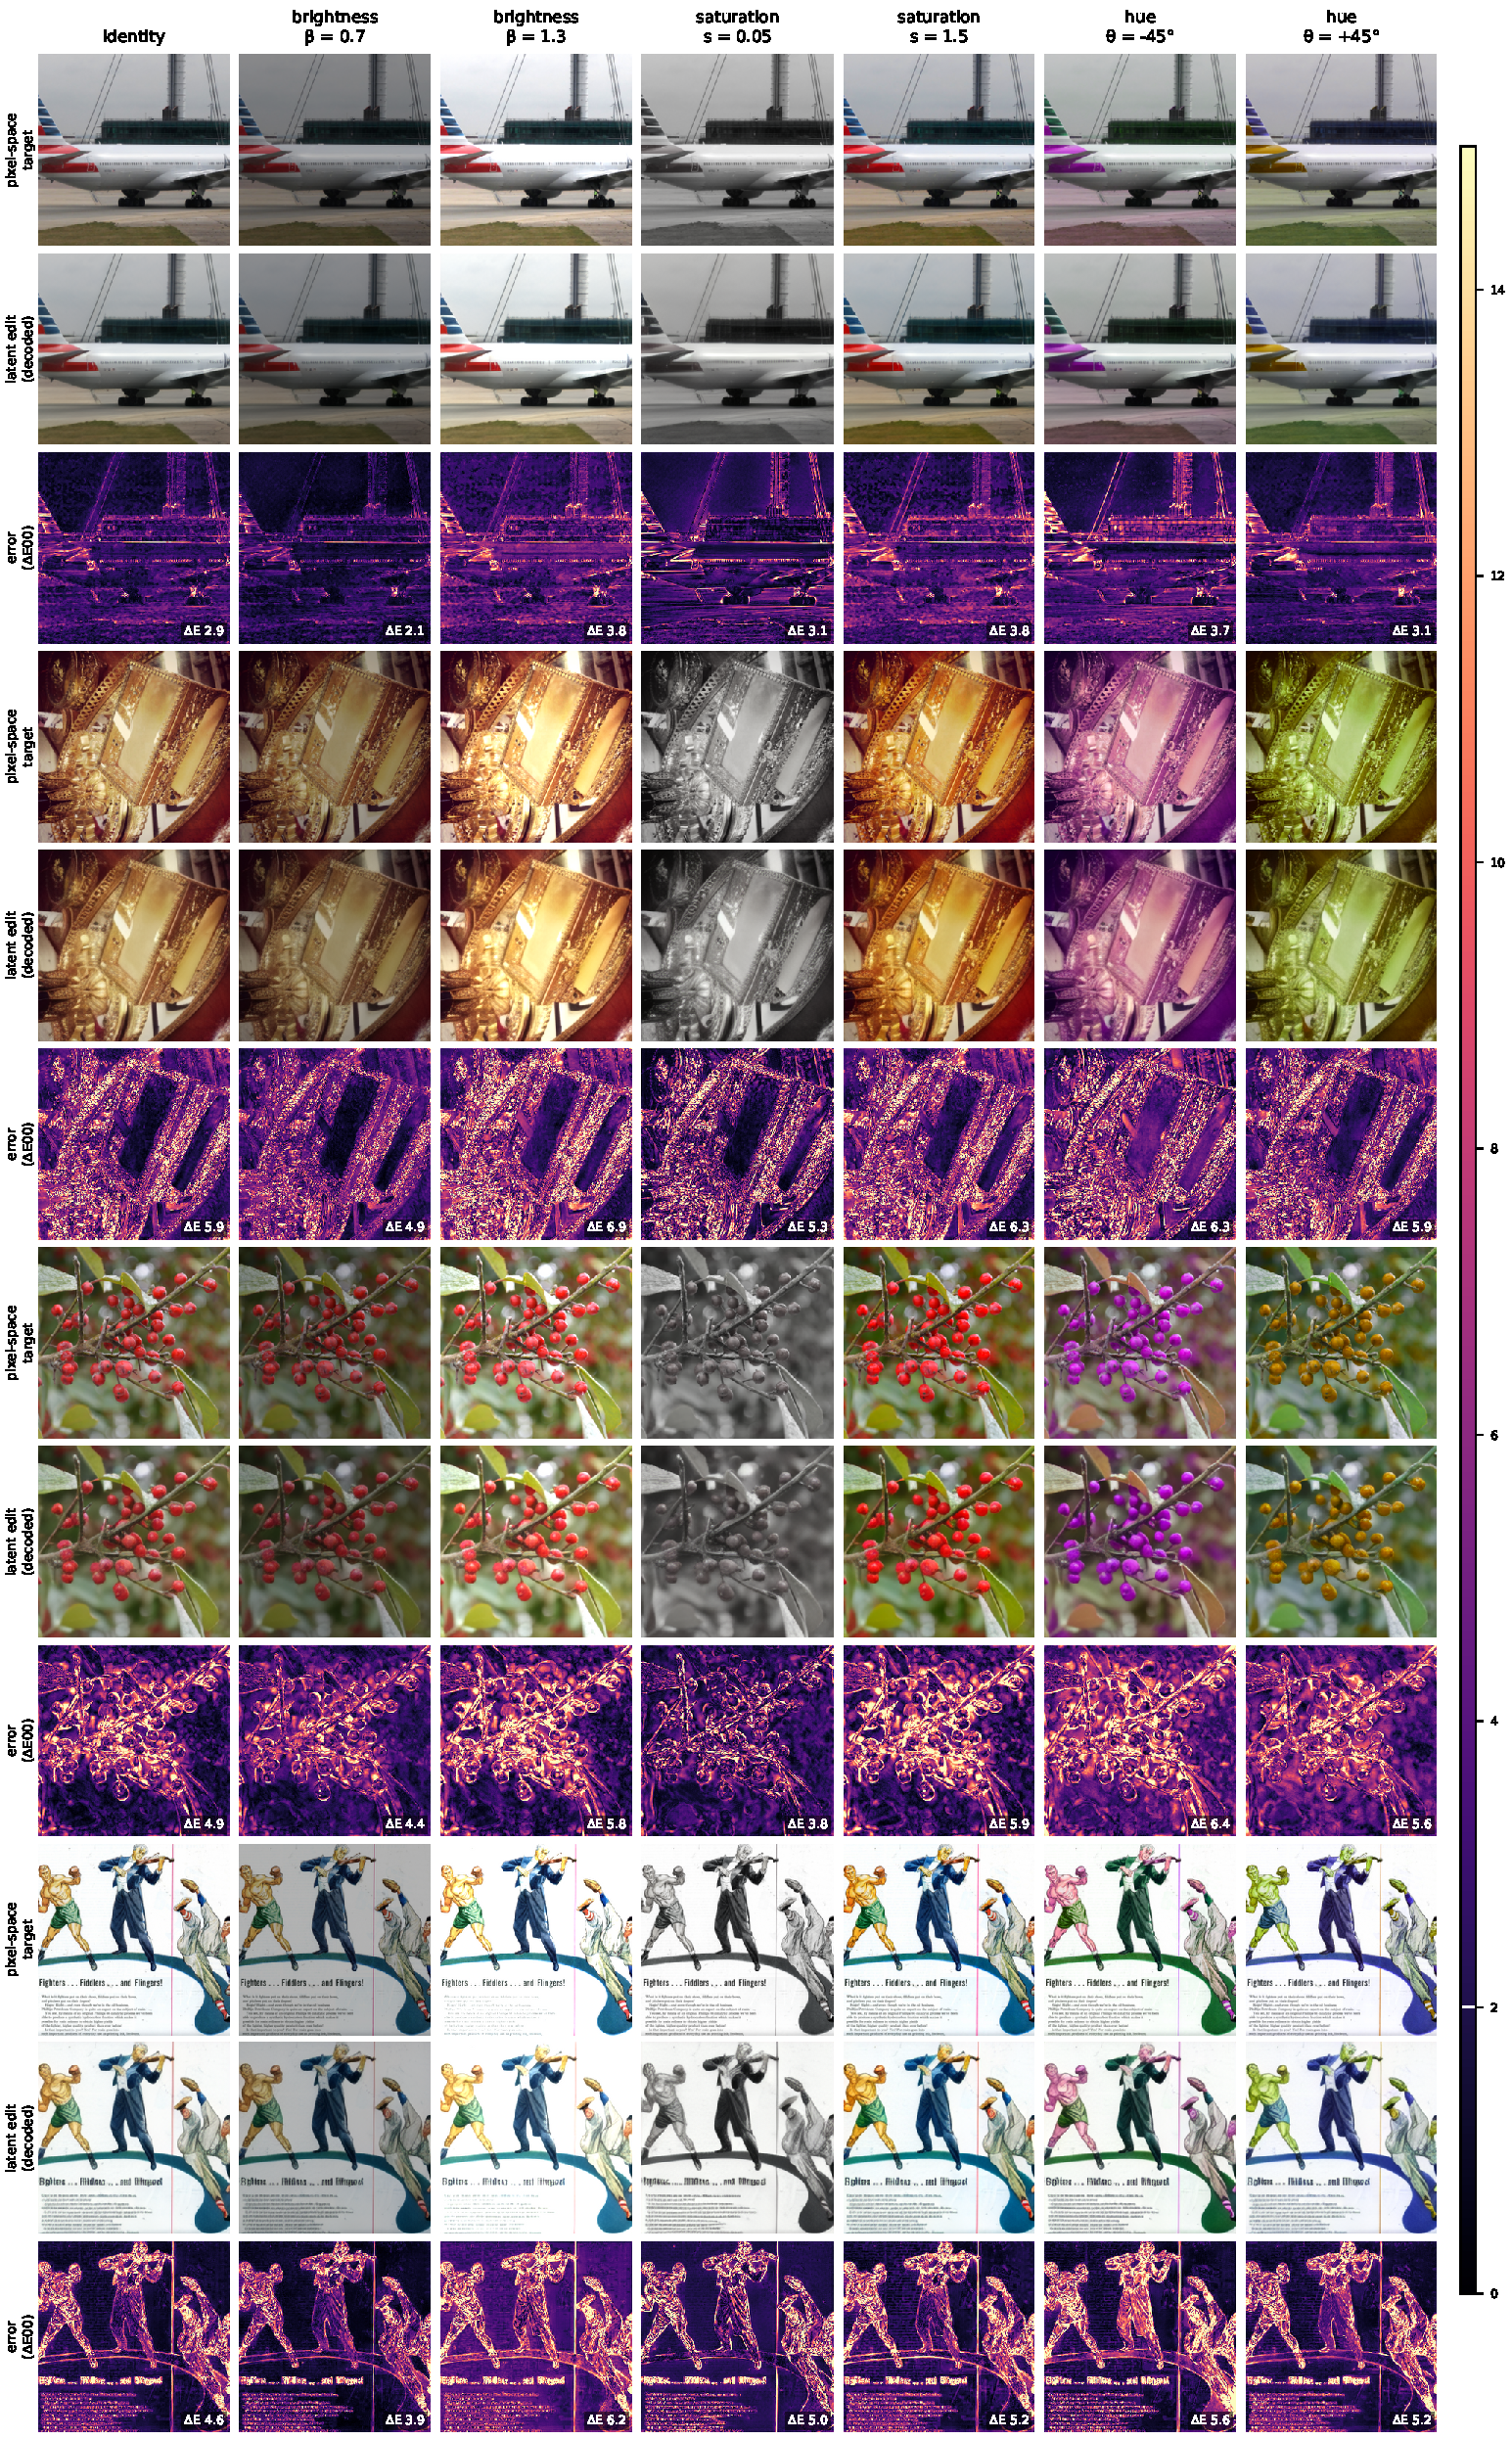
\includegraphics[width=\linewidth]{figures/fig1_editing.pdf}
\caption{Latent-space color editing with the closed-form operator on the
fine-tuned tokenizer: each column applies Eq.~\eqref{eq:closedform} for the
labeled transform directly to the latent before decoding.}
\end{figure}}{%
\noindent\fbox{\parbox{\linewidth}{\textbf{Figure pending:} generate with
\texttt{scripts/make\_fig1\_editing.py} on the cluster (see
\texttt{paper/README.md}).}}}

\end{document}
